\documentclass[compress]{beamer} %en animé
%\documentclass[trans]{beamer} %en superposé

%%%%%%%%%%%%%% LES PACKAGES
%================== ENCODAGE & LANGUE ==================
\usepackage[utf8]{inputenc}
\usepackage[T1]{fontenc}
%\usepackage[french]{babel} % Optionnel

%================== MATHS & SYMBOLES ===================
\usepackage{amsmath, amssymb, amsfonts}
\usepackage{yhmath, mathdots, cancel}
\usepackage{siunitx}
\usepackage{gensymb}
\usepackage{textcomp}
\usepackage{pifont}
\usepackage{xspace}


%================== TABLEAUX ============================
\usepackage{array, tabularx, multirow, booktabs}

%================== COULEURS & GRAPHISMES ===============
\usepackage{color}
\usepackage{tikz}
\usetikzlibrary{
  shapes.geometric,
  backgrounds,
  fadings,
  patterns,
  shadows.blur,
  shapes,
  positioning,
  decorations.pathreplacing,
  matrix
}
\usepackage{tikz-3dplot}
\usepackage{asymptote}
\usepackage{xcolor}

%================== MISE EN PAGE ========================
\usepackage{changepage}
\usepackage{calc}
\usepackage{caption}
\usepackage{xspace}
\usepackage{ragged2e}
\usepackage{amsmath, amsfonts, mathtools, amsthm, amssymb}
\usepackage{adjustbox}
\usepackage{caption}
\usepackage{beamerappendixnote}
\usepackage{bookmark}


%================== ALGORITHMIQUE =======================
\usepackage[ruled,vlined]{algorithm2e}
\SetAlgorithmName{Algorithme}{Algo}{Liste des algorithmes}
\SetFuncArgSty{textup}
\SetArgSty{textup}
\SetKwFor{ForEach}{pour tout}{faire}{}
\SetKwFor{For}{pour}{faire}{finpour}
\SetKwIF{Si}{SinonSi}{Sinon}{si}{alors}{sinon si}{sinon}{}
\SetKwInput{Input}{Entrée}
\SetKwInput{Output}{Sortie}
\SetKwProg{myproc}{Procédure}{:}{}
\SetKw{Return}{retourner}
\SetKwComment{tcc}{(*}{*)}
\SetKwFor{Tq}{tant que}{faire}{}
\SetKwRepeat{Repeter}{répéter}{jusqu’à}
\renewcommand{\thealgocf}{}
%================== AUTRES ==============================
\usepackage[clock]{ifsym}


%%%%%%%%%%%%%% THEME BEAMER
%votre nom court qui apparaîtra dans l'en tête
\newcommand{\initiales}{Lucie-Hélène CUINGNET }
\usetheme{CambridgeUS}
\usecolortheme{seahorse}


%--------marges
\setbeamersize{text margin left= 0.7cm}
\setbeamersize{text margin right= 0.7cm}

%--------tête et pieds
\setbeamertemplate{navigation symbols}{}
\setbeamertemplate{footline}[frame number]
\setbeamertemplate{headline}{
  %la premiere ligne
  	\begin{beamercolorbox}[ht=0.42cm, vmode]{section in head/foot}
	\hspace{0.4cm} \insertshorttitle 
	\hspace*{0.1cm}- \initiales - {\insertshortdate}
	\vspace*{0.08cm} 
  	\end{beamercolorbox}
  %la deuxième ligne
	\begin{beamercolorbox}[ht=0.4cm, vmode]{subsection in head/foot}
	%titre de la section si elle est pas 0
		\ifnum\value{section}=0{} 
		\else{ \hspace{0.8cm} \thesection - \insertsectionhead }
		\fi
	%séparateur + titre de la sous-section si elle est pas 0
		\ifnum\value{subsection}=0{} 
		\else{ 
			\hspace*{0.1cm} \couleur{$\bullet$} \hspace*{0.1cm} 
			\thesection.\thesubsection \, \insertsubsectionhead
		}
		\fi
		\vspace*{0.12cm}
\end{beamercolorbox}
%\vspace*{-0.03cm} %pour pas qu'il y ait d'espace avec la ligne de frametitle
 }
%\setbeamertemplate{frametitleheigth}{4cm}
\setbeamertemplate{frametitle}{
	\vspace*{-0.04cm} 
	\begin{beamercolorbox}[ht=0.8cm,wd=\paperwidth, vmode]{frametitle}
		\hspace{0.3cm} \insertframetitle \vspace*{0.1cm}
	\end{beamercolorbox}
}

%commande pour ajuster l'alignement vertical des titres sans lettres descendantes
%\newcommand{\esp}{\\[0.1cm]} %--version qui marche sans le package minted
\newcommand{\esp}{\\[-0.5cm]} %--version qui marche avec le package minted


%--------couleurs
\setbeamercolor{structure}{fg=turquoiseFonce!70!black} 

\setbeamercolor{block title}{fg=turquoiseFonce!70!black,bg=vertdEau}
\setbeamercolor{block body}{bg=vertdEau!10!white}

\setbeamercolor{block title alerted}{bg=vertdEau!85!white,fg=turquoiseFonce!80!black}
\setbeamercolor{block body alerted}{bg=vertdEau!8!white}
%\setbeamercolor{alerted text}{fg=red}

\setbeamercolor{block title example}{bg=vertdEau,fg=turquoiseFonce}
\setbeamercolor{block body example}{bg=vertdEau!10!white}
\setbeamercolor{example text}{fg=blue!20!turquoise}

%-------- TOC
\setbeamertemplate{section in toc}[sections numbered]

%-----------------------------------------------
%Plan qui s'affiche au début de chaque section %|
\AtBeginSection[]{                             %|
\begin{frame}[plain]                           %|
\frametitle{Plan\\[0.1cm]}                     %|
\tableofcontents[                              %|
currentsection,                                %|
hideothersubsections,                          %|
subsubsectionstyle=hide]                       %|
\addtocounter{framenumber}{-1}                 %|
\end{frame}}                                   %|
%-----------------------------------------------




%-------- commande pour les ref sur les slides
\newcommand{\bandeauREF}[1]{
\noindent\makebox[\textwidth][l]{%
\hspace{-\dimexpr\oddsidemargin+1in}%
\colorbox{expli!20!white}{%
\parbox{\dimexpr\paperwidth-2\fboxsep}{
\footnotesize\textcolor{expli!80!black}{#1}
}}}}
% Commandes utilitaires
\tikzset{every picture/.style={line width=0.75pt}} %set default line width to 0.75pt        
\newcommand{\imageFrame}{
  \draw [line width=0.75] (261.98,12.03) -- (262.02,142.84) -- (150.52,236.47) -- (150.47,105.66) -- cycle ;
}
\newcommand{\lin}[1]{\texttt{#1}} % Évite minted si pas nécessaire
\newcommand{\flch}{\item[$\rightarrow$]}
\newcommand{\dc}{{\usebeamercolor[fg]{structure}$\hookrightarrow$}}
\newcommand{\ok}{\textcolor{green}{\checkmark}}
\newcommand{\point}{{\usebeamercolor[fg]{structure}$\bullet\enskip$}}
\newcommand{\Point}{\point}
\newcommand{\couleur}[1]{{\usebeamercolor[fg]{structure}#1}}
\newcommand{\important}[1]{\couleur{\textbf{#1}}}
\newcommand{\remarque}[1]{\textit{\textrm{#1}}}
\newcommand{\cmark}{\ding{51}\xspace} % check ✓
\newcommand{\xmark}{\ding{55}\xspace} % cross ✗


%%%%%%%%%%%%%% MA PALETTE DE COULEURS
%%%%%%%%%%%%%% couleurs locales
\newcommand{\cearly}{orange!50!oranger}
\newcommand{\ctardy}{orange!50!oranger!50!magenta!50!violet}
\newcommand{\cmilieu}{yellow!45!magenta}
\newcommand{\cfenetre}{yellow!45!magenta}
%\newcommand{\cfenetre}{orange!80!magenta!80!violet}
\newcommand{\caxe}{blue!60!black}

\definecolor{vert}{RGB}{194, 247, 50}
\definecolor{vertClair}{RGB}{80, 180, 33}
\definecolor{vertFonce}{RGB}{20, 148, 20} 


\definecolor{turquoiseFonce}{RGB}{0, 149, 182} 
\definecolor{turquoise}{RGB}{0, 204, 203}
%\definecolor{turquoise}{RGB}{53, 123, 153} 
\colorlet{monCyan}{turquoise!90!blue} 

\colorlet{vertdEau}{blue!50!green!30!white} 

\definecolor{prec}{RGB}{128, 0, 128} 
\definecolor{hyp}{RGB}{255, 0, 127} 


\definecolor{orange}{RGB}{250, 130, 1}
\definecolor{orange1}{RGB}{244, 142, 3}
\definecolor{orange2}{RGB}{255, 195, 0}
%\colorlet{orangé}{orange!55!yellow}
\colorlet{oranger}{orange!55!yellow}
\definecolor{jaune}{RGB}{255, 195, 0 }
\colorlet{ocre}{orange!90!green!80!white} 


\definecolor{briqueRouge}{RGB}{200, 48, 24}
\definecolor{brique}{RGB}{141, 48, 24}
\definecolor{brown}{RGB}{165, 137, 107}
\definecolor{chamois}{RGB}{200, 141, 75}

\colorlet{lavande}{vertdEau!50!blue}
\definecolor{lilas}{RGB}{154, 107, 165}
\colorlet{parme}{magenta} %violet!30!magenta
\definecolor{mauve}{RGB}{161, 132, 220}%{147, 112, 219}

\definecolor{prunelle}{RGB}{106,24, 141}
\definecolor{prune}{RGB}{121, 7, 123}
\definecolor{violet}{RGB}{153, 0, 139}
\definecolor{violette}{RGB}{128, 0, 128} 

\definecolor{rose}{RGB}{255, 0, 127} 
\definecolor{framboise}{RGB}{141, 24, 59}
\colorlet{grenat}{magenta!90!red!80!black}

\colorlet{expli}{gray}

\definecolor{hellseahorse}{RGB}{204, 204, 255}
\definecolor{seahorse}{RGB}{204,180, 255}
\definecolor{darkseahorse}{RGB}{83, 74, 196}

%symboles pratiques
\newcommand{\flch}{\item[$\rightarrow$]}
\newcommand{\dc}{{\usebeamercolor[fg]{structure}$\hookrightarrow$}}
\newcommand{\ok}{\textcolor{vert}{\checkmark}}
\newcommand{\point}{{\usebeamercolor[fg]{structure}$\bullet\enskip$}}
\newcommand{\Point}{{\usebeamercolor[fg]{structure}$\bullet\enskip$}}


%styles
\newcommand{\couleur}[1]{{\usebeamercolor[fg]{structure}#1}}
\newcommand{\important}[1]{\couleur{\textbf{#1}}}
\newcommand{\remarque}[1]{\textit{\textrm{#1}}}

%pour le template
\newcommand{\lin}[1]{\mintinline{latex}{#1}}
%%%%%%%%%%%%%%%%%%%%%%%%%%%%%%%%%%%%%%%%%%%%%%%%%
\begin{document}
%

%%%%%%%%%%%%%%%%%%%%%%%%%%%%%%%%%%%%%%%%%%%%%%%%%
% A COMPLETER 
%%%%%%%%%%%%%%%%%%%%%%%%%%%%%%%%%%%%%%%%%%%%%%%%%

%entre crochet le titre court pour l'en tête puis le vrai titre
\title[Gros titre : et sous titre (version courte)]{
Reconstruction 3D :\\
{\large Comment reconstruir un objet en 3D à partir d'images ? }
}

\author{
\large 
Présentation de \important{Lucie-Hélène CUINGNET}\\[0.2cm]
\footnotesize
travail réalisé avec \couleur{Barnabé BARUCHEL}\\[0.4cm]
\vspace*{-1.2cm}
} 

%entre crochet la short date pour l'en-tête
\date[Juillet 2024]{}

\institute{}


%------------------------------------------------
\begin{frame}[plain]
\titlepage 
\addtocounter{framenumber}{-1} 
\end{frame}

%------------------------------------------------
\title[Gros titre : et sous titre (version courte)]{
Une page de titre avec logos :\\
{\large mais sans les affectations détaillées des auteurs }
}

%------------------------------------------------


% %%%%%%%%%%%%%%%%%%%%%%%%%%%%%%%%%%%%%%%%%%%%%%%%%
\section[Première section]{Première section : le haut des slides}
%------------------------------------------------
\begin{frame}
\frametitle{Titre d'une slide avant la sous-section\esp}
	Ici on n'a pas encore de titre de sous-section dans le badeau du haut.
	\label{slides_hors_subsec}
\end{frame}


%++++++++++++++++++++++++++++++++++++++++++++++++
\subsection{À propos de l'en-tête}
%++++++++++++++++++++++++++++++++++++++++++++++++
\begin{frame}
\frametitle{Titre d'une slide dans la sous-section\esp}
	Ici on a un titre de sous-section, contrairement à la slide~\ref{slides_hors_subsec}\\[2cm]
	Regarder le code ici pour référencer une slide avec \lin{\label} et la citer avec son numéro grâce à \lin{\ref}
\end{frame}


%------------------------------------------------
\begin{frame}
\frametitle{Ce qui apparaît dans l'en-tête}
	Dans la \important{première ligne}:
	\begin{itemize}
	\flch la version courte du titre, précisée en option  de  \lin{\title}\\
	\remarque{( en option = entre crochets, avant les accolades)}
	\flch la version courte du nom, voire des initiales, redéfinir la commande
	\lin{\newcommand{\initiales}{Petit Nom}} 
	\flch la version courte de la date, précisée en option de \lin{\date}\\
	\end{itemize}
	\bigskip
	Dans la \important{deuxième ligne}:
	\begin{itemize}
	\flch le numéro et le titre de la section, sauf si le numéro est nul\\
	\remarque{s'il est précisé en option de} \lin{\section}
	\remarque{le titre court est utilisé}
	\flch le numéro et le titre de la sous-section, sauf si le numéro est nul\\
	\remarque{s'il est précisé en option de} \lin{\subsection}
	\remarque{le titre court est utilisé}
\end{itemize}

\end{frame}


%++++++++++++++++++++++++++++++++++++++++++++++++
\subsection{Mise en forme du bandeau de titre}
%------------------------------------------------
\begin{frame}
\frametitle{Titre de la slide sans lettre descendant sous la baseline}
	Pour régler ce problème, utiliser la commande \lin{\esp} à la fin du titre, \textit{Cf.} slide suivante
\end{frame}


%------------------------------------------------
\begin{frame}
\frametitle{Titre de la slide sans lettre descendant sous la baseline\esp}
	Ici c'est mieux non?
\end{frame}


%------------------------------------------------
\begin{frame}[fragile]
\frametitle{Titre de la slide qui marche tout seul grâce au q et au g}
\end{frame}

% %%%%%%%%%%%%%%%%%%%%%%%%%%%%%%%%%%%%%%%%%%%%%%%%%
\section{Le corps des diapositives}

%++++++++++++++++++++++++++++++++++++++++++++++++
\subsection{Équations et formules}
%------------------------------------------------
\begin{frame}
	\frametitle{Suite d'équations avec \lin{align*}}
	\begin{align*}
		a 
		& = b+c+d * \sum_{i=1}^n x_i\\
		& = b+c+d * \sum_{i=1}^n (z_i - y_i)\\
		& \leqslant B+c+d * \sum_{i=1}^n (z_i - y_i) & 
		\textcolor{expli}{\textit{ ici une petite explication}}\\
	\end{align*}
\end{frame}

%------------------------------------------------
\begin{frame}
	\frametitle{Formules centrées, éventuellement encadrées\esp}
	Voilà une formule juste centrée car entre \lin{$$} et \lin{$$} 
	$$ A  = \sum_{i=1}^{n} a_i +b_i$$
	Voilà une formule encadrée avec \lin{\fbox} et centrée 
	\begin{center}
		\fbox{$\Delta^{early}_u\!(E,\!T) \!\geqslant 0$ if $u \in E$}
	\end{center}
	
	Voilà une formule encadrée en couleurs avec \lin{\fcolorbox} et centrée
	\begin{center}
		\fcolorbox{turquoiseFonce}{white}{$\Delta^{early}_u\!(E,\!T) \!\geqslant 0$ if $u \in E$}
	\end{center}
	NB: le deuxième argument de \lin{\fcolorbox} fixe la couleur du fond, je déconseille de l'utiliser avec une couleur franche, ainsi on évitera ça : 
	\fcolorbox{red}{blue}{$\Delta^{early}_u\!(E,\!T) \!\geqslant 0$ if $u \in E$} 
	et même
	\fcolorbox{green}{yellow}{$\Delta^{early}_u\!(E,\!T) \!\geqslant 0$ if $u \in E$} 
\end{frame}

%++++++++++++++++++++++++++++++++++++++++++++++++
\subsection{Environnements \lin{description} et \lin{minipage}}
%------------------------------------------------
\begin{frame}
  \frametitle{Exemples d'utilisation de l'environnement \lin{description}}
  On peut par exemple décrire le problème...
  \begin{description}
    \item[entrées:] première donnée\\
    deuxième donnée\\
    dernière donnée\\
    \item[sortie:] le résultat
  \end{description}
\end{frame}

%------------------------------------------------
\begin{frame}
  \frametitle{Exemples d'utilisation de l'environnement \lin{minipage}}
  
  \begin{minipage}{0.48\textwidth}
    Là, à gauche, une colonne qui fait presque la moitié de la slide, dans laquelle je peux écrire plein de choses et dont je peux constater la largeur complète grâce à 
    \lin{\hrule} \hrule
  \end{minipage}
  \hspace*{0.2cm}
  \begin{minipage}{0.48\textwidth}
    \hrule
    Là, à droite, une colonne qui fait presque la moitié de la slide, dans laquelle je peux écrire plein de choses et dont je peux constater la largeur grâce à \lin{\hrule}
    que j'ai mis cette fois en début de paragraphe
  \end{minipage}

  \vspace*{0.4cm}

  \begin{minipage}[t]{0.64\textwidth}
    NB: par défaut, l'alignement vertical des minipages est "centré", ce qu'on peut modifier avec l'option \lin{[t]}. 
    Ici on est entre \lin{\begin{minipage}[t]{0.64\textwidth}}
    et \lin{\end{minipage}}
  \end{minipage}
  \hspace*{0.2cm}
  \begin{minipage}[t]{0.32\textwidth}
    Ici une petite largeur donc peu de mots font vite une grande hauteur,
    Remarquez que bien que plus haute, le haut de cette mini-page est aligné avec celui de celle de gauche
  \end{minipage}
\end{frame}

%------------------------------------------------
\begin{frame}
  \frametitle{Attention avec \lin{minipage} sous beamer}
  
  \begin{minipage}{0.6\textwidth}
  	Comme on peut le voir ici, la somme des largeurs indiquées dans les minipage doit être moins que  \lin{\textwidth}, sans quoi la dernière minipage est renvoyée à la ligne comme on peut le voir ici où on a juxtaposé une \lin{{minipage}{0.6\textwidth}} et une \lin{{minipage}{0.4\textwidth}}.
  \end{minipage}
  \begin{minipage}{0.4\textwidth}
    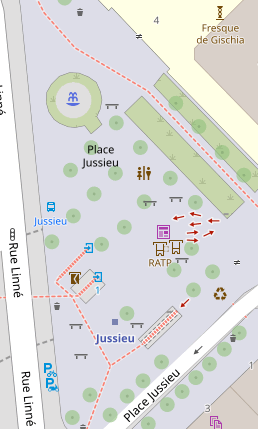
\includegraphics[scale=0.45]{pour_exemples/mini_plan.png}
  \end{minipage}
\end{frame}


%++++++++++++++++++++++++++++++++++++++++++++++++
\subsection{Minipages et inclusions (code, image)}
%------------------------------------------------
\begin{frame}
  \frametitle{Du texte et une image côte à côte}
  
  \begin{minipage}{0.56\textwidth}
    Lorem ipsum dolor sit amet, consectetuer adipiscing elit. 
    Ut purus elit, vestibulum ut, placerat ac, adipiscing vitae, felis. 
    Curabitur dictum gravida mauris. 
    Nam arcu libero, nonummy eget, consectetuer id, vulputate a, magna. 
    Donec vehicula augue eu neque. 
    Pellentesque habitant morbi tristique senectus et netus et malesuada fames ac turpis egestas. 
    Mauris ut leo. Cras viverra metus rhoncus sem. 
    Nulla et lectus vestibulum urna fringilla ultrices.
    Phasellus eu tellus sit amet tortor gravida placerat. Integer sapien est,
    iaculis in, pretium quis, viverra ac, nunc.
  \end{minipage}
  \hfill
  \begin{minipage}{0.38\textwidth}
    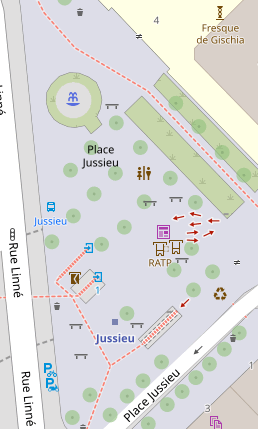
\includegraphics[scale=0.45]{pour_exemples/mini_plan.png}
  \end{minipage}
\end{frame}

%------------------------------------------------
\begin{frame}
  \frametitle{Du texte et du code C côte à côte\esp}
  
  \begin{minipage}{0.4\textwidth}
    Lorem ipsum dolor sit amet, consectetuer adipiscing elit. 
    Ut purus elit, vestibulum ut, placerat ac, adipiscing vitae, felis. 
    Curabitur dictum gravida mauris. 
    Nam arcu libero, nonummy eget, consectetuer id, vulputate a, magna. 
    Donec vehicula augue eu neque. 
  \end{minipage}
  \begin{minipage}{0.58\textwidth}
    \inputminted[firstline=3, lastline=8,firstnumber=1]{c}{pour_exemples/main.c}
  \end{minipage}
\end{frame}

%------------------------------------------------
\begin{frame}
  \frametitle{Une image et du code Ocaml côte à côte\esp}
  
  \begin{minipage}{0.28\textwidth}
    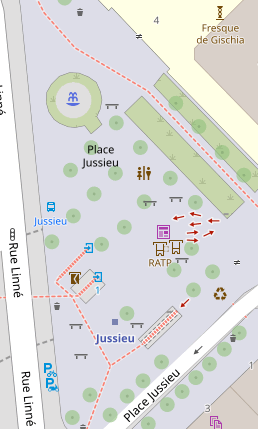
\includegraphics[scale=0.35]{pour_exemples/mini_plan.png}
  \end{minipage}
  \begin{minipage}{0.68\textwidth}
    \inputminted[firstline=1, lastline=10,firstnumber=1]{ocaml}{pour_exemples/test.ml}
  \end{minipage}
\end{frame}

%------------------------------------------------
\begin{frame}
  \frametitle{Deux images côte à côte}

  \begin{minipage}{0.49\textwidth}
	  \begin{figure}
		  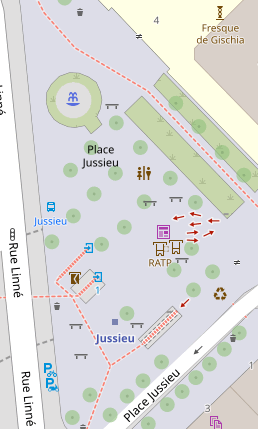
\includegraphics[scale=0.35]{pour_exemples/mini_plan.png}
		  \caption*{Une première image : un plan}
	  \end{figure}
  \end{minipage}
  \hfill
  \begin{minipage}{0.49\textwidth}
    \begin{figure}
		  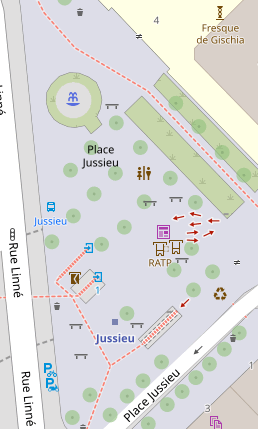
\includegraphics[scale=0.35]{pour_exemples/mini_plan.png}
		  \caption*{Une deuxième image : la même}
	  \end{figure}
  \end{minipage}
\end{frame}

%++++++++++++++++++++++++++++++++++++++++++++++++
\subsection{Une diapositive avec du pseudo-code}
%------------------------------------------------
\begin{frame}
	\small
	\frametitle{Pseudo-code avec \lin{algorithm} du package \lin{algo2e}}
	\begin{algorithm}[H]
		\caption{\textsf{Dijkstra}}
		\Input{Un graphe pondéré $G = (S, A,c)$ où $c : A \rightarrow \mathbb{R}^{+}$, $s\!\in\! S$}
		\Output{La distance de $s$ à chaque sommet de $S$}
		\BlankLine
		Initialiser $\delta[u]$ à $+\infty$ pour $u \in S$\;
 		Initialiser $\pi[u]$ à $\textsf{??}$ pour $u \in S$\;
  		$\delta[s] \gets 0$\;
  		%{\footnotesize\tcc*{~La source est à distance 0 d'elle-même }}	
 		$\pi[s] \gets s$\;
 		%{\footnotesize\tcc*{~La source est la racine de l’arborescence }}
  		$\textsf{todo} \gets \{s\}$\;
  		%{\footnotesize\tcc*{~La racine est le premier sommet à traiter }}
  		\Tq{$\textsf{todo} \neq \emptyset$}{
   			 Soit $u \in \textsf{todo}$ minimisant $\delta[u]$\;
    			\ForEach{$v \in \textsf{voisin}(u)$}{ 
    				$\textsf{Relacher}(G, u, v ,\delta, \pi, \textsf{todo})$
   			}
    			Ôter $u$ de $\textsf{todo}$ \;
  		}	
 	\Return{$\delta$}
\end{algorithm}
\end{frame}

%++++++++++++++++++++++++++++++++++++++++++++++++
\subsection{Astuces pour s'étaler en largeur}
%------------------------------------------------
\begin{frame}
  \frametitle{Moins de marge (ou plus?)}

  \begin{adjustwidth}{-1.5 em}{-1.5em}
    Ce paragraphe est entre 
    \lin{\begin{adjustwidth}{-1.5 em}{-1.5em}} et \lin{\end{adjustwidth}}
    ce qui lui permet de s'étaler  d'un bout à l'autre de la slide.
    En fait on a réduit les marges à gauche et à droite de 1.5em,
    on peut aussi augmenter les marges (réduire la largeur du texte donc) en mettant des valeurs positives, cf paragraphe juste après
  \end{adjustwidth}
  
  \bigskip
  
  \begin{adjustwidth}{2 em}{5em}
    Ce paragraphe est entre 
    \lin{\begin{adjustwidth}{2 em}{5em}} et \lin{\end{adjustwidth}}
    ce qui lui permet de s'étaler sur une largeur plus petite,et décalée vers la gauche.
    En fait on a augmenté la marge à gauche de 2em, et celle à droite de 5em
  \end{adjustwidth}
\end{frame}





%%%%%%%%%%%%%%%%%%%%%%%%%%%%%%%%%%%%%%%%%%%%%%%%%
\section[Première section]{Première section : le haut des slides}
%------------------------------------------------
\begin{frame}
\frametitle{Titre d'une slide avant la sous-section\esp}
	Ici on n'a pas encore de titre de sous-section dans le badeau du haut.
	\label{slides_hors_subsec}
\end{frame}


%++++++++++++++++++++++++++++++++++++++++++++++++
\subsection{À propos de l'en-tête}
%++++++++++++++++++++++++++++++++++++++++++++++++
\begin{frame}
\frametitle{Titre d'une slide dans la sous-section\esp}
	Ici on a un titre de sous-section, contrairement à la slide~\ref{slides_hors_subsec}\\[2cm]
	Regarder le code ici pour référencer une slide avec \lin{\label} et la citer avec son numéro grâce à \lin{\ref}
\end{frame}


%------------------------------------------------
\begin{frame}
\frametitle{Ce qui apparaît dans l'en-tête}
	Dans la \important{première ligne}:
	\begin{itemize}
	\flch la version courte du titre, précisée en option  de  \lin{\title}\\
	\remarque{( en option = entre crochets, avant les accolades)}
	\flch la version courte du nom, voire des initiales, redéfinir la commande
	\lin{\newcommand{\initiales}{Petit Nom}} 
	\flch la version courte de la date, précisée en option de \lin{\date}\\
	\end{itemize}
	\bigskip
	Dans la \important{deuxième ligne}:
	\begin{itemize}
	\flch le numéro et le titre de la section, sauf si le numéro est nul\\
	\remarque{s'il est précisé en option de} \lin{\section}
	\remarque{le titre court est utilisé}
	\flch le numéro et le titre de la sous-section, sauf si le numéro est nul\\
	\remarque{s'il est précisé en option de} \lin{\subsection}
	\remarque{le titre court est utilisé}
\end{itemize}

\end{frame}


%++++++++++++++++++++++++++++++++++++++++++++++++
\subsection{Mise en forme du bandeau de titre}
%------------------------------------------------
\begin{frame}
\frametitle{Titre de la slide sans lettre descendant sous la baseline}
	Pour régler ce problème, utiliser la commande \lin{\esp} à la fin du titre, \textit{Cf.} slide suivante
\end{frame}


%------------------------------------------------
\begin{frame}
\frametitle{Titre de la slide sans lettre descendant sous la baseline\esp}
	Ici c'est mieux non?
\end{frame}


%------------------------------------------------
\begin{frame}[fragile]
\frametitle{Titre de la slide qui marche tout seul grâce au q et au g}
\end{frame}

%%%%%%%%%%%%%%%%%%%%%%%%%%%%%%%%%%%%%%%%%%%%%%%%%
\section{Faire des animations}

%------------------------------------------------
\begin{frame}
  \frametitle{Pourquoi des animations ?}
  
  \begin{itemize}
   \flch Faire des animations sur une diapositive permet que son contenu arrive progressivement, de manière synchrone avec votre discours.
  Cela évite que votre public lise une formule compliquée encadrée en fin de diaopositive au lieu de vous écouter expliquer le début de la diapositive.\\
  \flch Dans le cas où vous avez fait une simulation dynamique, cela permet de simuler un petit dessin animé dans un fichier pdf autorisé aux concours.
  \end{itemize}
\end{frame}

%++++++++++++++++++++++++++++++++++++++++++++++++
\subsection{Sur une diapo quelconque}
%------------------------------------------------
%\begin{frame}
%	\frametitle{Suite d'équations animée avec \lin{\pause}}
%	On reprend la suite d'équations présentée plus haut, mais grâce à des commandes \lin{\pause}, celles-ci apparaissent au fur et à mesure.
%	\begin{align*}
%	  \pause
%		a \pause
%		& = b+c+d * \sum_{i=1}^n x_i \pause \\
%		& = b+c+d * \sum_{i=1}^n (z_i - y_i) \pause \\
%		& \leqslant B+c+d * \sum_{i=1}^n (z_i - y_i) & \pause
%		\textcolor{expli}{\textit{ ici une petite explication}}\\
%	\end{align*}
%\end{frame}


%------------------------------------------------
\begin{frame}
	\frametitle{Formules au fur et à mesure avec \lin{\pause}}
	On reprend la suite d'équations présentée plus haut, mais grâce à des commandes \lin{\pause}, celles-ci apparaissent au fur et à mesure.
	\pause
	Voilà une formule juste centrée car entre \lin{$$} et \lin{$$} 
	$$ A  = \sum_{i=1}^{n} a_i +b_i$$
	
	\pause
	Voilà une formule encadrée avec \lin{\fbox}et centrée 
	\begin{center}
		\fbox{$\Delta^{early}_u\!(E,\!T) \!\geqslant 0$ if $u \in E$}
	\end{center}
	\pause
	
	Voilà une formule encadrée en couleurs avec \lin{\fcolorbox} et centrée
	\begin{center}
		\fcolorbox{turquoiseFonce}{white}{$\Delta^{early}_u\!(E,\!T) \!\geqslant 0$ if $u \in E$}
	\end{center}
\end{frame}

%------------------------------------------------
\begin{frame}
  \frametitle{Exemple avec \lin{\only}}

  \only<1>{N'apparaît que sur la slide "1", grâce à \lin{\only<1>{...}},\\
  puis disparaît et laisse sa place.\\
  }
  \couleur { partie là tout le temps}, car hors d'un \texttt{$\backslash$only<1>}\\

  \only<2-4>{N'apparaît que sur les slides "2", "3" et "4",
  grâce à \texttt{$\backslash$only<2-4>\{...\}},\\
  puis disparaît et laisse sa place.\\
  }

  \only<2>{N'apparaît que sur la slide "2", grâce à \texttt{$\backslash$only<2>\{...\}},\\
  puis disparaît et laisse sa place.\\
  }

  \only<3->{Apparaît de la slide "3" à la fin, grâce à \texttt{$\backslash$only<3->\{...\}}, avant sa place n'est pas reversée
  }
\end{frame}


%------------------------------------------------
\begin{frame}
\frametitle{Exemple avec \lin{\onslide}}

\onslide<1>{N'apparaît que sur la slide "1", grâce à \texttt{$\backslash$onslide<1>\{...\}},\\
mais ici sa place est reversée, pas réutilisée.\\
}
\couleur { partie là tout le temps}, car hors d'un \texttt{$\backslash$onslide<1>}\\

\onslide<2-4>{N'apparaît que sur les slides "2", "3" et "4",
grâce à \texttt{$\backslash$only<2-4>\{...\}},\\
mais ici sa place est reversée, pas réutilisée.\\
}

\onslide<2>{N'apparaît que sur la slide "2", grâce à \texttt{$\backslash$onslide<2>\{...\}},\\
mais ici sa place est reversée, pas réutilisée.\\
}

\onslide<3->{Apparaît de la slide "3" à la fin, grâce à \texttt{$\backslash$onslide<3->\{...\}},
mais sa place est reversée, pas réutilisée.\\
}
\end{frame}



%++++++++++++++++++++++++++++++++++++++++++++++++
\subsection{Avec des images}
%------------------------------------------------
\begin{frame}
\frametitle{Images animées - exemple - le début à la main}
  \begin{figure}
	  \only<1>{
\includegraphics[scale=0.45]{pour_exemples/anim/img1.jpg}}
	  \only<2>{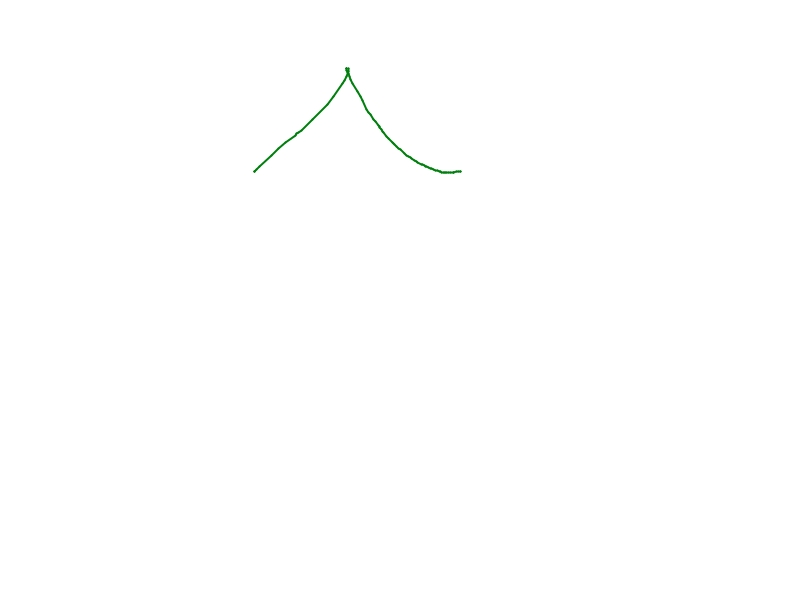
\includegraphics[scale=0.45]{pour_exemples/anim/img2.jpg}}
	  \only<3>{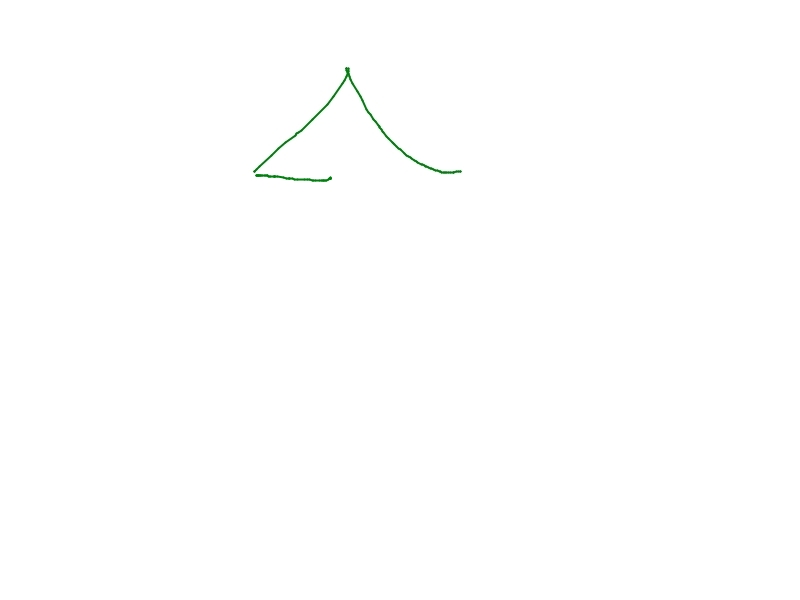
\includegraphics[scale=0.45]{pour_exemples/anim/img3.jpg}}
%	  \only<4>{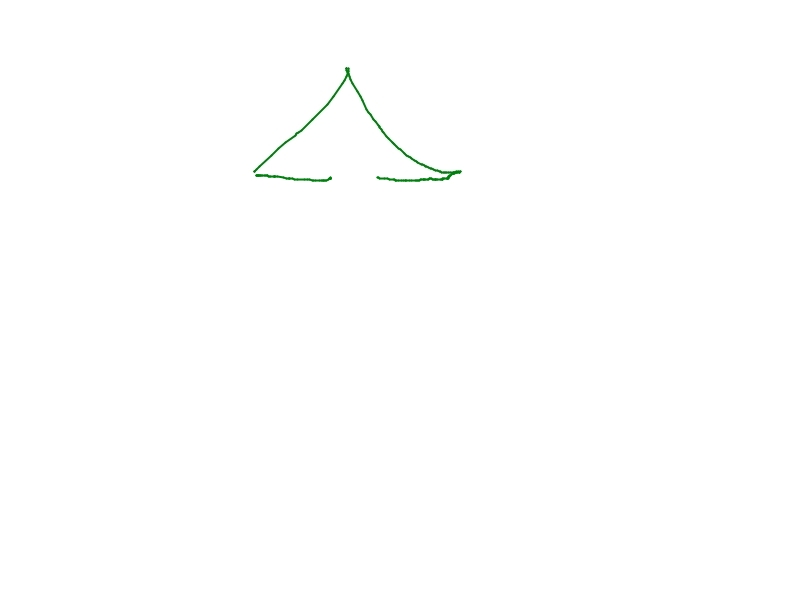
\includegraphics[scale=0.45]{pour_exemples/anim/img4.jpg}}
%	  \only<5>{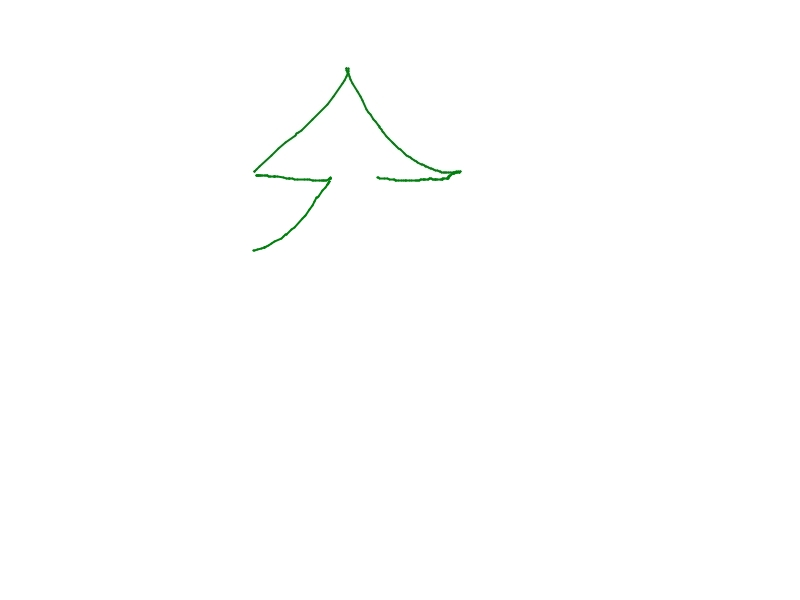
\includegraphics[scale=0.45]{pour_exemples/anim/img5.jpg}}
%	  \only<6>{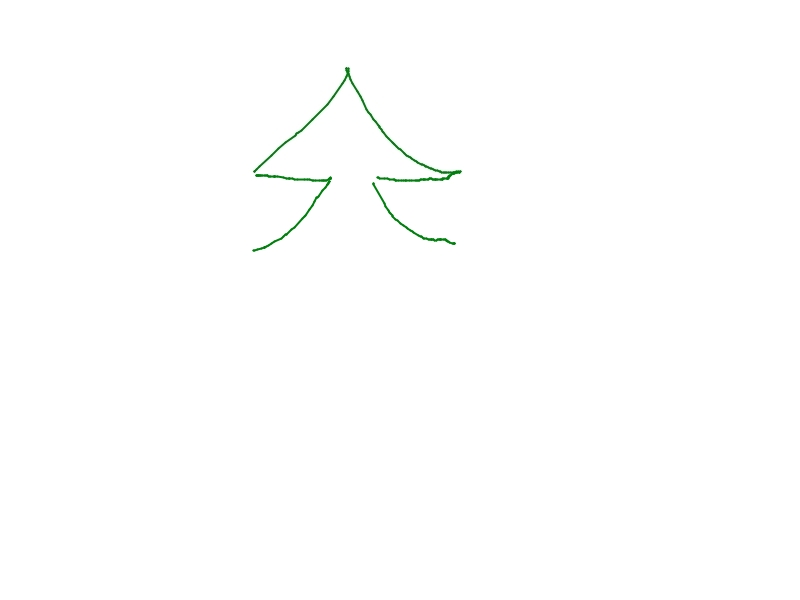
\includegraphics[scale=0.45]{pour_exemples/anim/img6.jpg}}
%	  \only<7>{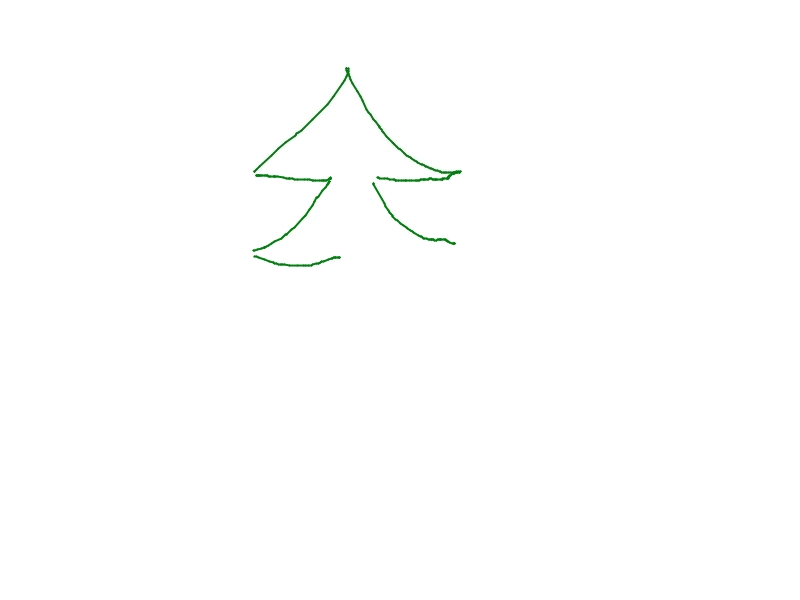
\includegraphics[scale=0.45]{pour_exemples/anim/img7.jpg}}
%	  \only<8>{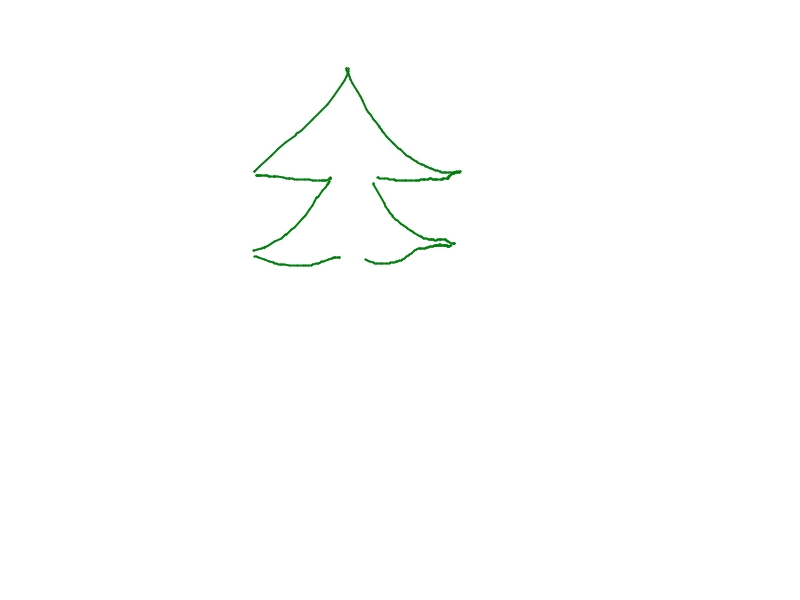
\includegraphics[scale=0.45]{pour_exemples/anim/img8.jpg}}
%	  \only<9>{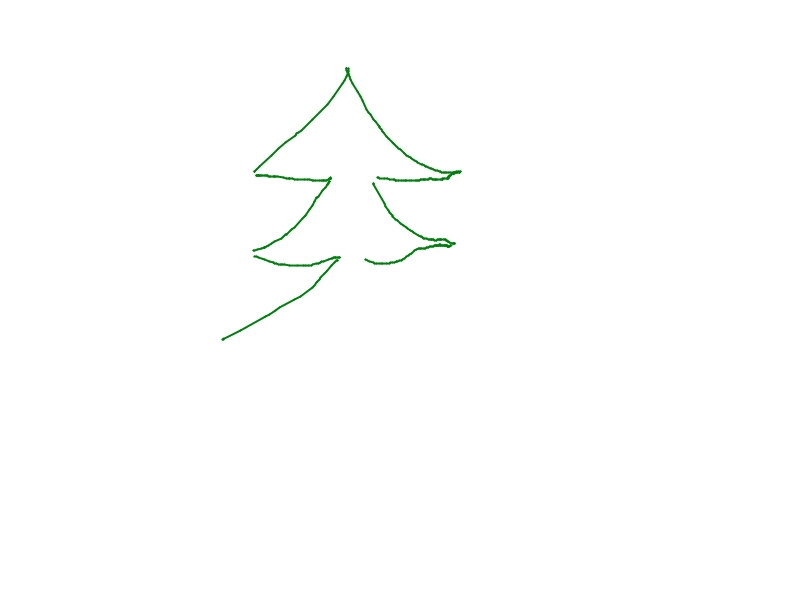
\includegraphics[scale=0.45]{pour_exemples/anim/img9.jpg}}
%	  \only<10>{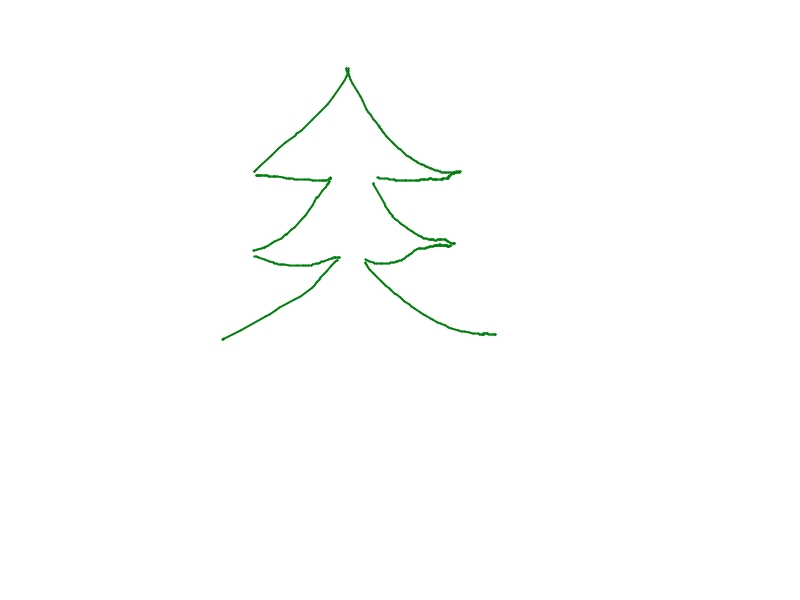
\includegraphics[scale=0.45]{pour_exemples/anim/img10.jpg}}
%	  \only<11>{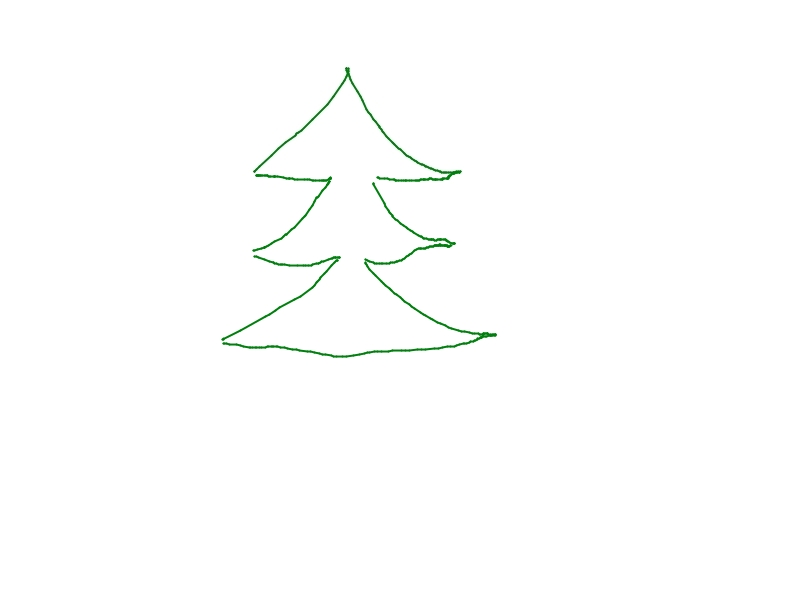
\includegraphics[scale=0.45]{pour_exemples/anim/img11.jpg}}
  \end{figure}
\end{frame}

%------------------------------------------------
\begin{frame}
  \frametitle{Images animées - exemple - le tout avec \lin{\foreach}}
  \begin{figure}
    \foreach \k in{1,2,...,11}{
	    \only<\k>{
	      {Image \k}
	      \includegraphics[scale=0.45]{pour_exemples/anim/img\k.jpg}
	    }
	  }
  \end{figure}
\end{frame}

%------------------------------------------------
\begin{frame}
  \frametitle{Images animées - explications}
  
  \begin{itemize}
    \flch On nomme les images à afficher successivement avec des noms comme \texttt{im1.jpg}, \texttt{im2.jpg}...
    où la numérotation suit bien sûr l'ordre dans lequel doivent apparaître ces images.
    \flch On peut alors faire des copier-coller de \lin{inludegraphics{im1.jpg}} en vhangeant le numéro, ou bien utiliser \lin{\foreach} pour faire une boucle
    \flch Attention le poids du PDF de présentation augmente très vite, or vous êtes limités en taille pour le PDF à envoyer aux concours (à 5Mo je crois).
    Vous pouvez commenter la slide qui inclut les 11 images du sapin, recompiler,  et observer que la taille du PDF a réduit d'un volume équivalent à la somme des 11 images (un peu plus même).
    Donc il faut avoir peu d'images (pas 50) ou des petites images, ou bien se mettre au tikz...
  \end{itemize}
\end{frame}




%++++++++++++++++++++++++++++++++++++++++++++++++
\subsection{Avec du tikz}
%------------------------------------------------
\begin{frame} [fragile]
  \frametitle{Exemple avec tikZ - v1}*
  
  On peut utiliser  \texttt{$\backslash$draw<n->} pour animer directement
  une figure tikz.\\[0.2cm]
  \alert{Attention}, la figure est replacée automatiquement à chaque étape en fonction de la place occupée par la figure à cette étape, donc si on veut voir le point bouger dans l'exemple ci-dessous, il faut un cadre fixe
  \begin{center}
    \begin{tikzpicture} 
    %cadre
    \draw[gray](0.5,-0.5)rectangle(6.5,0.5);
    %points
    \foreach \step in {1,2,3,...,8} {
      \draw<\step>(\step,0) node{$\bullet$};
    }
    \end{tikzpicture}
  \end{center}

\end{frame}

%------------------------------------------------
\begin{frame} [fragile]
  \frametitle{Exemple avec tikZ - v1}
  
  De plus, cet ajustement automatique rend parfois les animations désagréables,
  comme juste avant les deux derniers points qui ont tout fait bouger.
  Il faut donc mettre un cadre qui englobe la superposition de toutes les étapes.
  Exemple ci-dessous :
  \begin{center}
    \begin{tikzpicture} 
      %cadre
      \draw[gray](0.5,-0.5)rectangle(8.5,0.5);
      %points
      \foreach \step in {1,2,3,...,8} {
        \draw<\step>(\step,0) node{$\bullet$};
      }
    \end{tikzpicture}
  \end{center}

\end{frame}



%++++++++++++++++++++++++++++++++++++++++++++++++
\subsection{Animation et numérotation}
%------------------------------------------------
\begin{frame}
\frametitle{Animation et numérotation\esp}
	Comme on peut le voir sur les slides précédentes, il y a par défaut un seul numéro pour les différents slides issues des animations d'une seule "frame". 
	Autrement dit on a un numéro de slide pour chaque occurence d'un environnement \lin{frame}.
	\medskip
	
	Dans la plupart des cas ce comportement par défaut est opportun, mais dans le cas où l'on veut pouvoir faire référence à une étape précise de l'animation, comme dans un déroulé d'algorithme par exemple, on peut ajouter des numéros.
	Pour cela, on incrémente \textit{manuellement} le compteur \texttt{framenumber} grâce à la commande \lin{\addtocounter{framenumber}{1}}.
\end{frame}

%------------------------------------------------
\addtocounter{framenumber}{-1}
\begin{frame}
\frametitle{Numéroter chaque étape d'une animation avec \lin{\pause}}
 	\addtocounter{framenumber}{1}
	Si on utilise des \lin{\pause}, il suffit de mettre une seule fois l'incrémentation \lin{\addtocounter{framenumber}{1}} juste après le \lin{\begin{frame}} car elle est ré-évaluée pour chaque slide.
	Comme elle est évaluée la première fois alors que le \lin{\begin{frame}} incrémente déjà automatiquement ce compteur, on compense en décrémentant avant le \lin{\begin{frame}}.
	\medskip
	Exemple ici  : 
	\begin{itemize}
		\item étape 1 \pause
		\item étape 2 \pause
		\item étape 3 \pause
	\end{itemize}
	
\end{frame}

%------------------------------------------------
\addtocounter{framenumber}{-1}
\begin{frame}
\frametitle{Numéroter chaque étape d'une animation avec \lin{\only}}
 	\addtocounter{framenumber}{1}
 	Avec des  \lin{\only} ça marche pareil : il suffit de mettre une seule fois \lin{\addtocounter{framenumber}{1}} juste après le \lin{\begin{frame}} et une seule fois \lin{\addtocounter{framenumber}{-1}} juste avant.
	\medskip
	Exemple ici : 
	\begin{itemize}
		\only<1>{\item étape 1}
		\only<2->{\item étape 2 et suivantes}
		\only<3>{\item étape 3}
	\end{itemize}
\end{frame}

% \section{Troisième section : le bas des slides}
%++++++++++++++++++++++++++++++++++++++++++++++++
\subsection{Pour les références}
%------------------------------------------------
\begin{frame}[fragile]
\frametitle{Petit bandeau de citation d'une référence\esp}
	Se fait à la main en utilisant la commande \lin{\bandeauREF}.\\
	En plus il faut ajuster à la main un  \lin{\vspace} pour le forcer à être bien en bas... (\lin{\vfill}) ne marche pas).\\
	\vspace*{5cm}
	\bandeauREF{%
		\hspace*{0.2cm}\textbf{Auteur, 2020,} Journal Scientifique en Open Source, titre de l'article\\
		\hspace*{0.2cm}\textbf{Autrice, 2020,} Journal Scientifique en Open Source, titre de l'article\\
		\\
	} 
\end{frame}







%++++++++++++++++++++++++++++++++++++++++++++++++
\subsection{Numérotation}
%------------------------------------------------
\begin{frame}[fragile]
\frametitle{La numérotation des diapo\esp}
Compte les diapo sans multiplicité : si le contenu d'un diapo arrive petit à petit parce qu'on a utilisé des %\mintinline{latex}{pause} 
\\[1cm]
Ne compte pas la page de titre, ni les pages de plan. \\[1cm]
Compte le nombre total de slides\\[1cm]
Si vous avez n slides bonus, vous pouvez fausser (mais rectifier) 
le nombre total de slides avec  \lin{\addtocounter\{framenumber\}\{-n\} } 
\end{frame}


%------------------------------------------------
\begin{frame}[fragile]
\frametitle{La dernière vraie slide\esp}
\label{derniere_slide_effective}
Elle est donc numérotée \theframenumber / \theframenumber
\end{frame}


%------------------------------------------------
\begin{frame}[fragile]
\frametitle{Slide bonus qui ne compte pas}
Elle est donc numérotée \theframenumber / \ref{derniere_slide_effective}
\end{frame}


%------------------------------------------------
\begin{frame}[fragile]
\frametitle{Encore une slide bonus qui ne compte pas}
Elle est donc numérotée \theframenumber / \ref{derniere_slide_effective}
\end{frame}
\addtocounter{framenumber}{-2} 





\end{document}
